% Template for Cogsci submission with R Markdown

% Stuff changed from original Markdown PLOS Template
\documentclass[10pt, letterpaper]{article}

\usepackage{cogsci}
\usepackage{pslatex}
\usepackage{float}
\usepackage{caption}

% amsmath package, useful for mathematical formulas
\usepackage{amsmath}

% amssymb package, useful for mathematical symbols
\usepackage{amssymb}

% hyperref package, useful for hyperlinks
\usepackage{hyperref}

% graphicx package, useful for including eps and pdf graphics
% include graphics with the command \includegraphics
\usepackage{graphicx}

% Sweave(-like)
\usepackage{fancyvrb}
\DefineVerbatimEnvironment{Sinput}{Verbatim}{fontshape=sl}
\DefineVerbatimEnvironment{Soutput}{Verbatim}{}
\DefineVerbatimEnvironment{Scode}{Verbatim}{fontshape=sl}
\newenvironment{Schunk}{}{}
\DefineVerbatimEnvironment{Code}{Verbatim}{}
\DefineVerbatimEnvironment{CodeInput}{Verbatim}{fontshape=sl}
\DefineVerbatimEnvironment{CodeOutput}{Verbatim}{}
\newenvironment{CodeChunk}{}{}

% cite package, to clean up citations in the main text. Do not remove.
\usepackage{cite}

\usepackage{color}

% Use doublespacing - comment out for single spacing
%\usepackage{setspace}
%\doublespacing


% % Text layout
% \topmargin 0.0cm
% \oddsidemargin 0.5cm
% \evensidemargin 0.5cm
% \textwidth 16cm
% \textheight 21cm

\title{A Language's Unigram Entropy Distribution Predicts Self-Paced Reading
Times}


\author{{\large \bf Josef Klafka} \\ \texttt{jklafka@uchicago.edu} \\ Department of Psychology \\ University of Chicago \And {\large \bf Daniel Yurovsky} \\ \texttt{yurovsky@uchicago.edu} \\ Department of Psychology \\ University of Chicago}

\begin{document}

\maketitle

\begin{abstract}
The abstract should be one paragraph, indented 1/8 inch on both sides,
in 9 point font with single spacing. The heading Abstract should be 10
point, bold, centered, with one line space below it. This one-paragraph
abstract section is required only for standard spoken papers and
standard posters (i.e., those presentations that will be represented by
six page papers in the Proceedings).

\textbf{Keywords:}
Entropy; self-paced reading; information theory; language processing
\end{abstract}

\section{Uniform Information Density}\label{uniform-information-density}

The average distribution of information in English sentences-what is it?
Genzel \& Charniak (2002) looked at the log-probability of words
occurring in sentences as you proceed through a paragraph or article and
found that less common/less likely words occurred more frequently as you
moved through the text. The relationship they found was roughly an
affine linear function, leading them to propose the \emph{constant
entropy rate} (CER) principle: the entropy of words in a sentence,
i.e.~the uncertainty about what words will appear in a sentence, will
increase at a constant, linear rate through a paragraph. This idea was
used by Aylett \& Turk (2004), Levy \& Jaeger (2007) and Frank \& Jaeger
(2008) among others. The CER principle was adapted by Jaeger (2008) into
the \emph{uniform information density} (UID) principle: uniformation is
evenly spread throughout a sentence. From a theoretical standpoint, this
makes sense as the optimal distribution for information throughout a
sentence: if you miss any word I've said, the rest of the information in
the sentence is intact, and you lose no more than if you miss any other
word I'd have said. Description of the UID perspective and what it
predicts for entropy distributions and what that means.

\subsection{Yu challenge}\label{yu-challenge}

The UID perspective is challenged in Yu et al. (2016), by performing an
analysis of entropy by position in the text portion of the British
National Corpus. They use the following formula for each word position X
of sentences of fixed length k from the corpus, where each i is a word
occurring in position X and pi is the number of times word i occurs in
position X divided by the number of total words that occur in position X
i.e.~the number of sentences of length k.

\[H(X) = \sum\limits_w p(w)\log\big(p(w)\big)\] Yu et al. (2016) refer
to their distribution for English as a `three-step distribution':
relatively low entropy at the beginning of a sentence, then a jump, then
flat entropy in the middle, a dip before the final position and a jump
with the final word. View the figure below for a visual demonstration.

\begin{CodeChunk}
\begin{figure*}[h]

{\centering 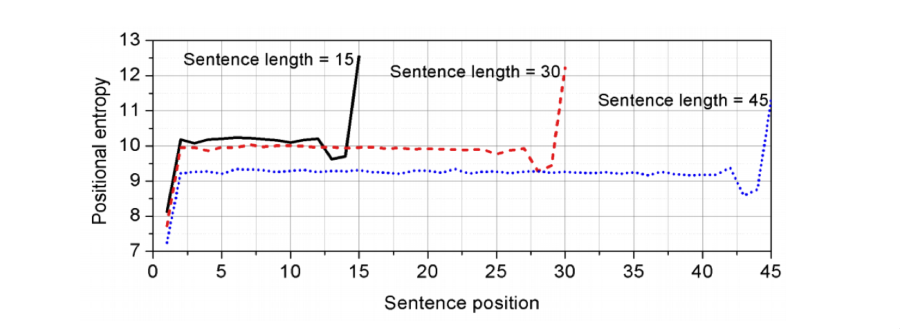
\includegraphics{figs/yunigram-1} 

}

\caption[English entropy distribution for three sentence lengths from BNC]{English entropy distribution for three sentence lengths from BNC}\label{fig:yunigram}
\end{figure*}
\end{CodeChunk}

This diverges from the UID account, which would predict a simple affine
function. Our replication with CHILDES. Conditional entropy and mutual
information. Link with Thiessen \& Onnis (to appear). Mention
Ferrer-i-Cancho (2017), which provides a theoretical basis for the end
of the sentence being the center of information. Cross-linguistic
variation. Our Wikipedia analysis Link with Kuperman et al. (2010).
Consequences for eye-tracking. Talk about Zhan and Levy (2018) and how
current work in eye-tracking and language processing disputes the UID
account. Our eye-tracking experiment.

\section{Formalities, Footnotes, and
Floats}\label{formalities-footnotes-and-floats}

Use standard APA citation format. Citations within the text should
include the author's last name and year. If the authors' names are
included in the sentence, place only the year in parentheses, as in
(1972), but otherwise place the entire reference in parentheses with the
authors and year separated by a comma (Newell \& Simon, 1972). List
multiple references alphabetically and separate them by semicolons
(Chalnick \& Billman, 1988; Newell \& Simon, 1972). Use the et. al.
construction only after listing all the authors to a publication in an
earlier reference and for citations with four or more authors.

For more information on citations in RMarkdown, see
\textbf{\href{http://rmarkdown.rstudio.com/authoring_bibliographies_and_citations.html\#citations}{here}.}

\subsection{Footnotes}\label{footnotes}

Indicate footnotes with a number\footnote{Sample of the first
footnote.} in the text. Place the footnotes in 9 point type at the
bottom of the page on which they appear. Precede the footnote with a
horizontal rule.\footnote{Sample of the second footnote.} You can also
use markdown formatting to include footnotes using this
syntax.\footnote{Sample of a markdown footnote.}

\subsection{Figures}\label{figures}

All artwork must be very dark for purposes of reproduction and should
not be hand drawn. Number figures sequentially, placing the figure
number and caption, in 10 point, after the figure with one line space
above the caption and one line space below it. If necessary, leave extra
white space at the bottom of the page to avoid splitting the figure and
figure caption. You may float figures to the top or bottom of a column,
or set wide figures across both columns.

\subsection{Two-column images}\label{two-column-images}

You can read local images using png package for example and plot it like
a regular plot using grid.raster from the grid package. With this method
you have full control of the size of your image. \textbf{Note: Image
must be in .png file format for the readPNG function to work.}

You might want to display a wide figure across both columns. To do this,
you change the \texttt{fig.env} chunk option to \texttt{figure*}. To
align the image in the center of the page, set \texttt{fig.align} option
to \texttt{center}. To format the width of your caption text, you set
the \texttt{num.cols.cap} option to \texttt{2}.

\begin{CodeChunk}
\begin{figure*}[h]

{\centering 
\includegraphics{figs/2-col-image-1} 

}

\caption[This image spans both columns]{This image spans both columns. And the caption text is limited to 0.8 of the width of the document.}\label{fig:2-col-image}
\end{figure*}
\end{CodeChunk}

\subsection{One-column images}\label{one-column-images}

Single column is the default option, but if you want set it explicitly,
set \texttt{fig.env} to \texttt{figure}. Notice that the
\texttt{num.cols} option for the caption width is set to \texttt{1}.

\begin{CodeChunk}
\begin{figure}[H]

{\centering 
\includegraphics{figs/image-1} 

}

\caption[One column image]{One column image.}\label{fig:image}
\end{figure}
\end{CodeChunk}

\subsection{R Plots}\label{r-plots}

You can use R chunks directly to plot graphs. And you can use latex
floats in the fig.pos chunk option to have more control over the
location of your plot on the page. For more information on latex
placement specifiers see
\textbf{\href{https://en.wikibooks.org/wiki/LaTeX/Floats,_Figures_and_Captions}{here}}

\begin{CodeChunk}
\begin{figure}[H]

{\centering 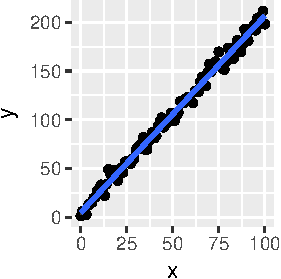
\includegraphics{figs/plot-1} 

}

\caption[R plot]{R plot}\label{fig:plot}
\end{figure}
\end{CodeChunk}

\subsection{Tables}\label{tables}

Number tables consecutively; place the table number and title (in 10
point) above the table with one line space above the caption and one
line space below it, as in Table 1. You may float tables to the top or
bottom of a column, set wide tables across both columns.

You can use the xtable function in the xtable package.

\begin{table}[H]
\centering
\begin{tabular}{rrrrr}
  \hline
 & Estimate & Std. Error & t value & Pr($>$$|$t$|$) \\ 
  \hline
(Intercept) & -0.02 & 0.10 & -0.2 & 0.82 \\ 
  x & 1.95 & 0.10 & 19.2 & 0.00 \\ 
   \hline
\end{tabular}
\caption{This table prints across one column.} 
\end{table}

\section{Acknowledgements}\label{acknowledgements}

Place acknowledgments (including funding information) in a section at
the end of the paper.

\section{References}\label{references}

\setlength{\parindent}{-0.1in} \setlength{\leftskip}{0.125in} \noindent

\hypertarget{refs}{}
\hypertarget{ref-ChalnickBillman1988a}{}
Chalnick, A., \& Billman, D. (1988). Unsupervised learning of
correlational structure. In \emph{Proceedings of the tenth annual
conference of the cognitive science society} (pp. 510--516). Hillsdale,
NJ: Lawrence Erlbaum Associates.

\hypertarget{ref-NewellSimon1972a}{}
Newell, A., \& Simon, H. A. (1972). \emph{Human problem solving}.
Englewood Cliffs, NJ: Prentice-Hall.

\end{document}
